% !TeX spellcheck = es_ES
\documentclass[a4paper, 11pt]{article}
\usepackage[table,xcdraw]{xcolor}
\usepackage{graphicx}
\usepackage{hyperref}
\usepackage{mathtools}
\usepackage{amsmath}
\usepackage[spanish, activeacute]{babel} %Definir idioma español
\usepackage[utf8]{inputenc} %Codificacion utf-8

\usepackage{geometry}
\geometry{left=2.5cm,right=2.5cm,top=2.5cm,bottom=2.5cm}

\DeclareMathOperator*{\argmax}{arg\,max}

\title{\Large{\textbf{Algoritmos de optimización para juego tipo Arkanoid}}}

\author{\textit{Francisco Rubin Capalbo}\\
		Universidad Politécnica de Valencia }

\date{\today}

\begin{document}
    
    \maketitle
    \section{Descripción del problema}
    Los videojuegos pueden servir como una plataforma de prueba excelente para algoritmos de inteligencia artificial. No sólo tenemos flexibilidad para establecer cualquier objetivo que queramos que el algoritmo resuelva, además las soluciones se pueden presentar de una manera visual que todo el mundo entiende. \\
    
    Con esto en mente, he desarrollado un juego basándome en el conocido Arkanoid \cite{arkanoid}, pero con una diferencia importante. En vez de utilizar una plataforma controlada por el jugador para dirigir la bola hacia el objetivo, éste debe colocar una cantidad limitada de bolas en el escenario, en la posición y dirección que desee (Figura \ref{fig:arkanoid_1}). Cuando se pulsa el botón de comenzar la partida, éstas se empiezan a mover hacia su objetivo, y ya no es necesaria ninguna interacción (Figura \ref{fig:arkanoid_2}). \\
    
    Este cambio hace más adecuado el uso de un algoritmo de optimización, ya que podemos limitar el problema a obtener una configuración inicial de bolas (cada una definida por un vector de posición y otro de dirección), en la que la puntuación sea superior, sin tener que meternos en un problema más complejo como sería el entrenamiento de una plataforma que dirija las bolas durante la partida.
    
    El objetivo del juego es destruir todos los ladrillos en el menor tiempo posible, con el mínimo número de bolas utilizadas.
    
    
     \begin{figure}[htb!]
     	 \begin{minipage}{0.4\textwidth}
     		\centering
     		
\includegraphics[scale=.5]{images/arkanoid_1}
     		\caption{Posición inicial, fase colocación}
     		\label{fig:arkanoid_1}
     	\end{minipage}\hfill
    	\begin{minipage}{0.4\textwidth}
    		\centering
    		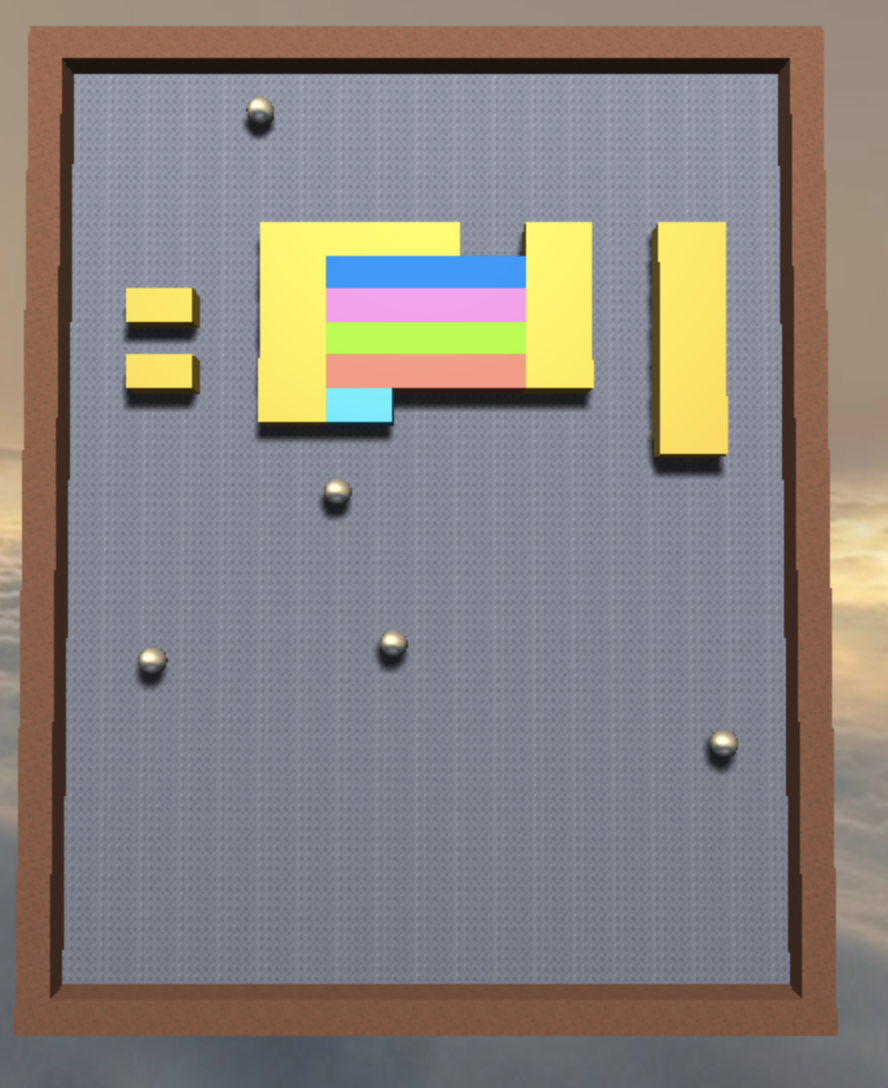
\includegraphics[scale=.5]{images/arkanoid_2}
    		\caption{Fase ejecución}
    		\label{fig:arkanoid_2}
    	\end{minipage}\hfill
    \end{figure}

	 	
\section{Métodos aplicados}
	Para resolver este problema de optimización he utilizado dos métodos dados en clases: Algoritmo genético y enfriamiento simulado.
	 	
 	\subsection{Fitness}
 		Ambos métodos requieren una función de fitness que evalúe la calidad de los individuos.
		En este caso cada individuo representa una configuración inicial del nivel, lo cual incluye una lista con configuraciones iniciales de bolas, en la que cada bola tiene una posición y una dirección. \\
 
		La función de fitness se calcula ejecutando una simulación del juego con dicha configuración inicial, y obteniendo algunos datos cuando la simulación termina: Número de bolas utilizadas y tiempo transcurrido. \\
		Hay que obtener un balance de estos dos valores para que los resultados no utilicen una cantidad exagerada de bolas para obtener un tiempo reducido, pero que tampoco aparezcan soluciones que tarden mucho utilizando sólo una bola. Tras hacer algunas pruebas, la función que he elegido es la siguiente:\\
		\begin{equation}
			fitness = numeroBolas * tiempoTranscurrido
		\end{equation}
		
		En este caso, cuanto menor sea el fitness, mejor es el resultado.

	\subsection{Algoritmo genético}
		
		Para este algoritmo es necesario definir una función de mutación y otra de cruce. 
				
		\subsubsection{Cruce}
			Con la función de cruce nos aseguramos que los individuos hijos obtengan parte de la configuración de sus dos padres, para que las configuraciones óptimas se mantengan. \\
			
			Lo que hacemos es asignar las bolas de ambos padres a los hijos, distribuidas de forma aleatoria. Po ejemplo, con dos padres con 5 bolas cada uno, podría salir un hijo de 1 bola y otro de 9 (aunque la probabilidad de que esto ocurra es reducida).
			
		\subsubsection{Mutación}
			La función de mutación realiza una pequeña modificación del individuo después de haber realizado el cruce, permitiendo una mayor exploración del espacio de búsqueda. \\
		
			En esta versión borramos una bola de la configuración con una probabilidad del 50\%, y añadimos otra nueva completamente diferente con la misma probabilidad. Esto permite que el número de bolas varíe y a la vez aparezcan nuevas bolas no vistas anteriormente.
			
		\subsubsection{Parámetros}
		
			A parte de las dos funciones, hay que especificar algunos parámetros: \\
			\begin{itemize}
				\item size: representa el número de individuos que se va a generar para cada generación
				\item steps: el número de generaciones que se crearán antes de dar por terminada la optimización
				\item keepBest: si el valor es true, indica que en cada generación se guardará el mejor individuo de la generación anterior, sin modificar
				\item randomChilds: si lo activamos, en cada generación se crearan 2 hijos aleatorios reusando el método 'seed', lo cual da más variedad a los resultados obtenidos y permite explorar nuevas soluciones
			\end{itemize}
		
		
	\subsection{Enfriamiento simulado}
		\subsubsection{Función de sucesor}
			Esta función define como se debe generar un posible sucesor de un individuo. La idea es que mantenga similitud a su vecino, pero que contenga algunas variaciones, que permiten explorar cambios que pueden mejorar el resultado.\\ 
				
			He hecho pruebas con dos funciones diferentes.\\ 
			
			La versión 1 es exactamente igual a la función de mutación del algoritmo genético. Un 50\% de probabilidad de borrar una bola, y un 50\% de añadir una nueva. De esta manera los vecinos van buscando pequeñas variaciones de bolas. \\
			
			La versión 2 intenta generar cambios mayores en los vecinos, como consecuencia de notar mucho estancamiento en la versión 1. Básicamente lo que hago es dar una probabilidad baja a cada bola de que se modifique completamente por otra aleatoria. Esto hace posible que más de una bola cambie en cada vecino, lo que nos puede llevar a nuevas combinaciones interesantes.

		\subsubsection{Parámetros}
			
			\begin{itemize}
				\item initialTemperature: temperatura inicial
				\item maxIterations: el número de vecinos que se crearán antes de dar por terminada la optimización
				\item coolingFactor: el factor por el que la temperatura se multiplica en cada cambio de vecino
			\end{itemize}

\section{Implementación de algoritmos}
	He implementado ambos algoritmos en Javascript, ya que las simulaciones son ejecutadas en una página web utilizando el motor gráfico para la web ThreeJS (basado en WebGL). Para conseguir una simulación rápida, las simulaciones se ejecutan en un hilo diferente al de renderizado (web worker), y no renderizan nada.  \\
	
	Como javascript es un lenguaje basado en eventos, he tenido que usar promesas, que se completan en cada iteración de los algoritmos. \\
	
	A parte de estos detalles, las implementaciones son muy similares a las de otras librerías, por lo que no me voy a extender explicándolas. \\ 
\section{Evaluación y discusión}
	He implementado más de 20 niveles diferentes en el juego, pero para la evaluación de los algoritmos me voy a centrar en el nivel 20, ya que sería un comparación injusta si mezclara diferentes niveles. \\
	
	Utilizaré dos métricas para la evaluación: Simulaciones ejecutadas y fitness obtenido. Normalmente es importante también el tiempo de cómputo, pero en este caso el número de simulaciones ejecutadas es más representativo, ya que el tiempo de cómputo de cada simulación varía mucho, independientemente de si el algoritmo es bueno o no. Esto se debe a que las soluciones con menos bolas utilizadas suelen tardar más tiempo, y requieren un cómputo superior. Utilizar el número de simulaciones ejecutadas es una manera de normalizar el tiempo de cómputo. \\
	
	Para mostrar los resultados utilizaré gráficas que muestran la progresión de el fitness (eje y) por el número de simulaciones ejecutadas (eje x). \\
	
	\subsection{Parametrización algoritmos genéticos}
		A continuación se pueden ver las 3 parametrizaciones diferentes del algoritmo genético utilizadas. La versión normal, la versión con randomChilds activado, y la versión con keepBest activado.  \\
		\begin{figure}[htb!]
			\begin{minipage}{0.8\textwidth}
				\centering
				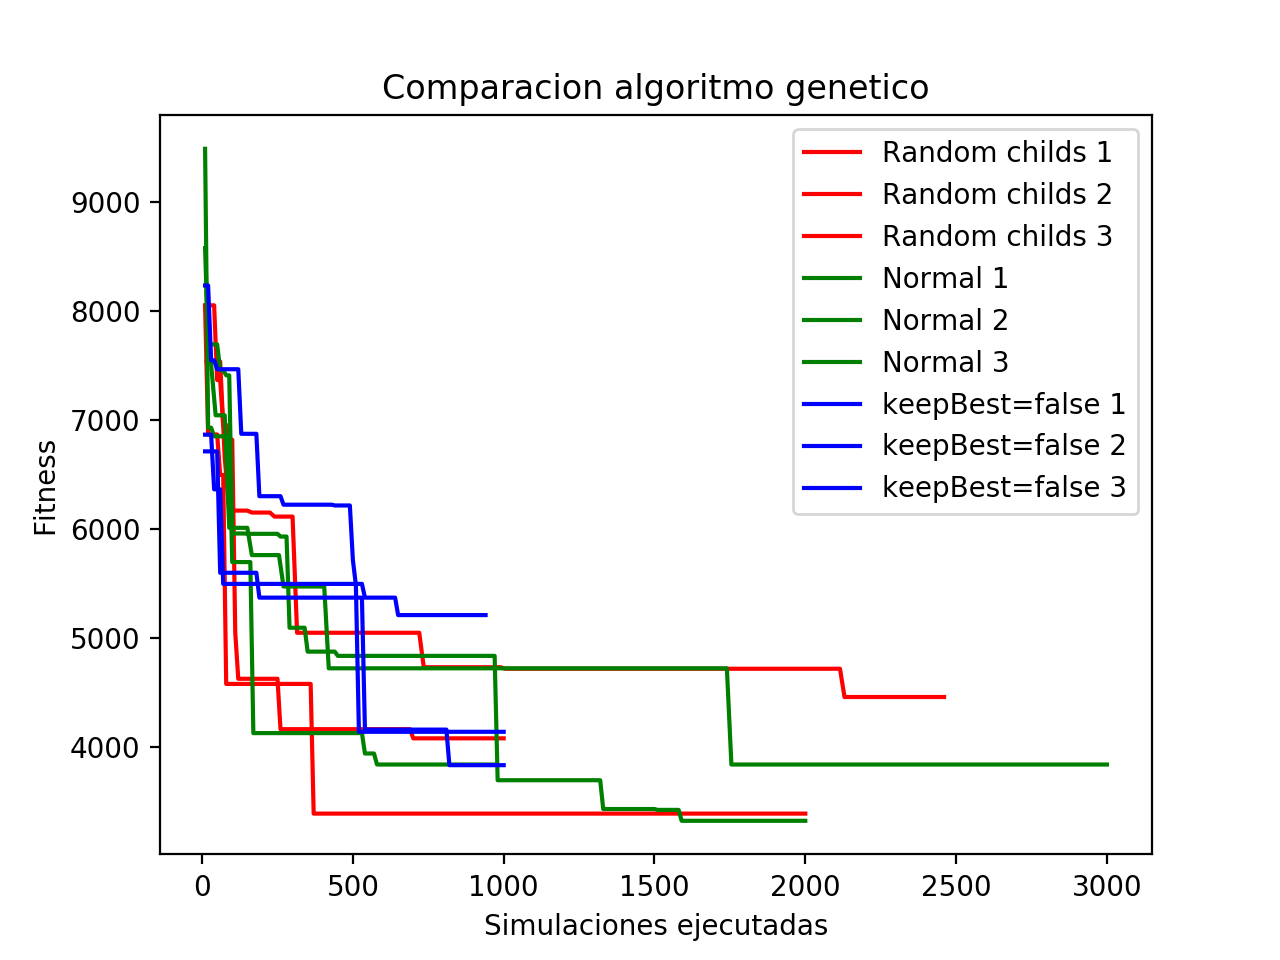
\includegraphics[scale=1]{images/comparacion_gen}
				\label{fig:comparacion_gen}
			\end{minipage}\hfill
		\end{figure}

		Como podemos observar, no hay una diferencia notable entre las 3 variantes. Las diferencias más marcadas se obtienen de una ejecución a otra, sin importar la parametrización. 

	\subsection{Parametrización enfriamiento simulado}
		Para enfriamiento simulado he probado con 2 alternativas, cada una con una versión de los algoritmos sucesor mencionados anteriormente. \\
		\begin{figure}[htb!]
			\begin{minipage}{0.8\textwidth}
				\centering
				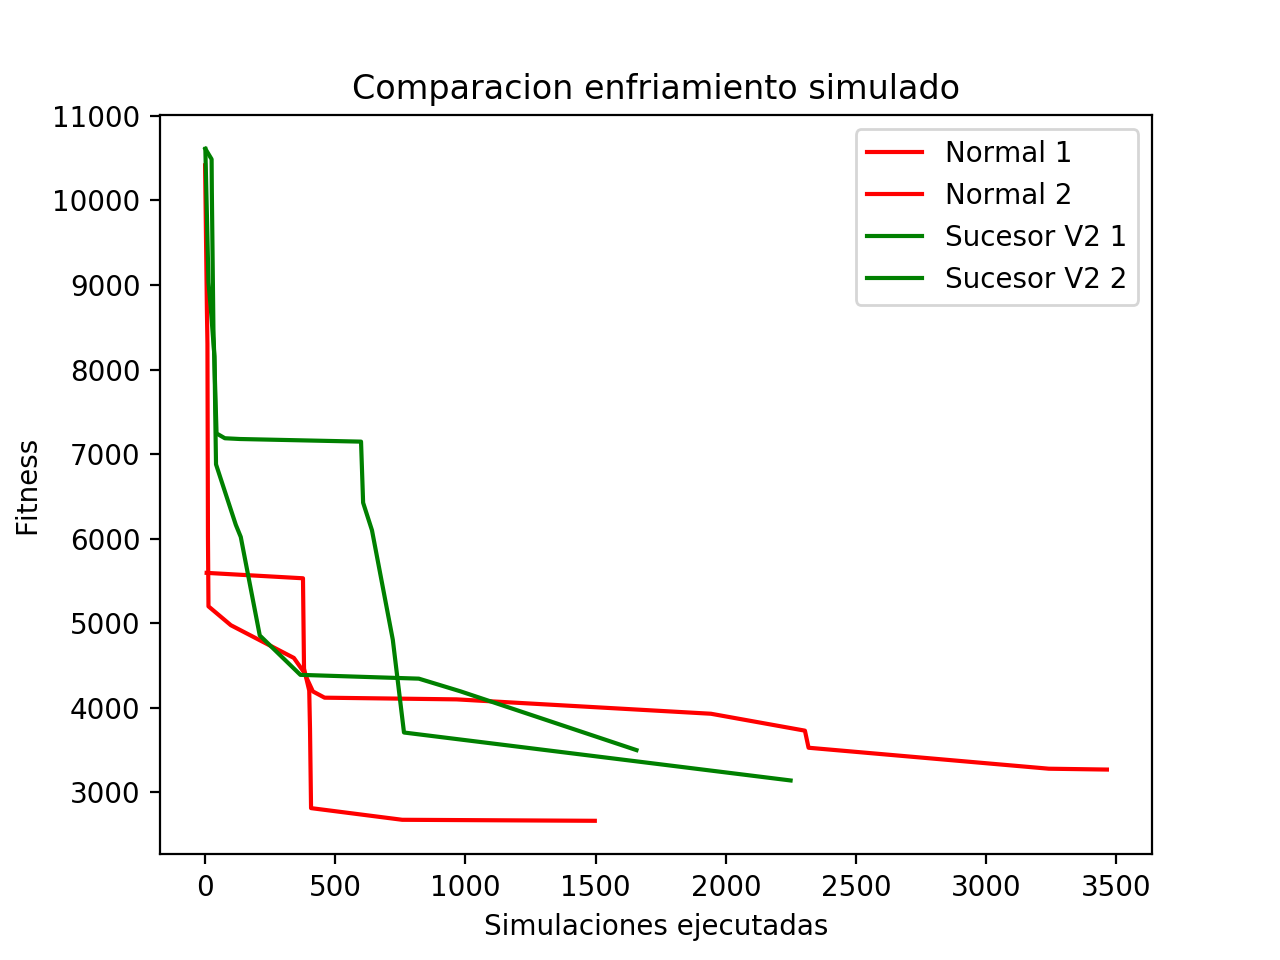
\includegraphics[scale=1]{images/comparacion_sim}
				\label{fig:comparacion_sim}
			\end{minipage}\hfill
		\end{figure}
		Las observaciones no son concluyentes, pero aquí tampoco parece haber mucha diferencia entre las dos alternativas. 
		
		\clearpage
	 \subsection{Comparación}
	 	Por último vamos a comparar nuestros resultados de enfriamiento simulado con los del algoritmo genético. \\ 
	 	
	 		\begin{figure}[htb!]
	 		\begin{minipage}{0.8\textwidth}
	 			\centering
	 			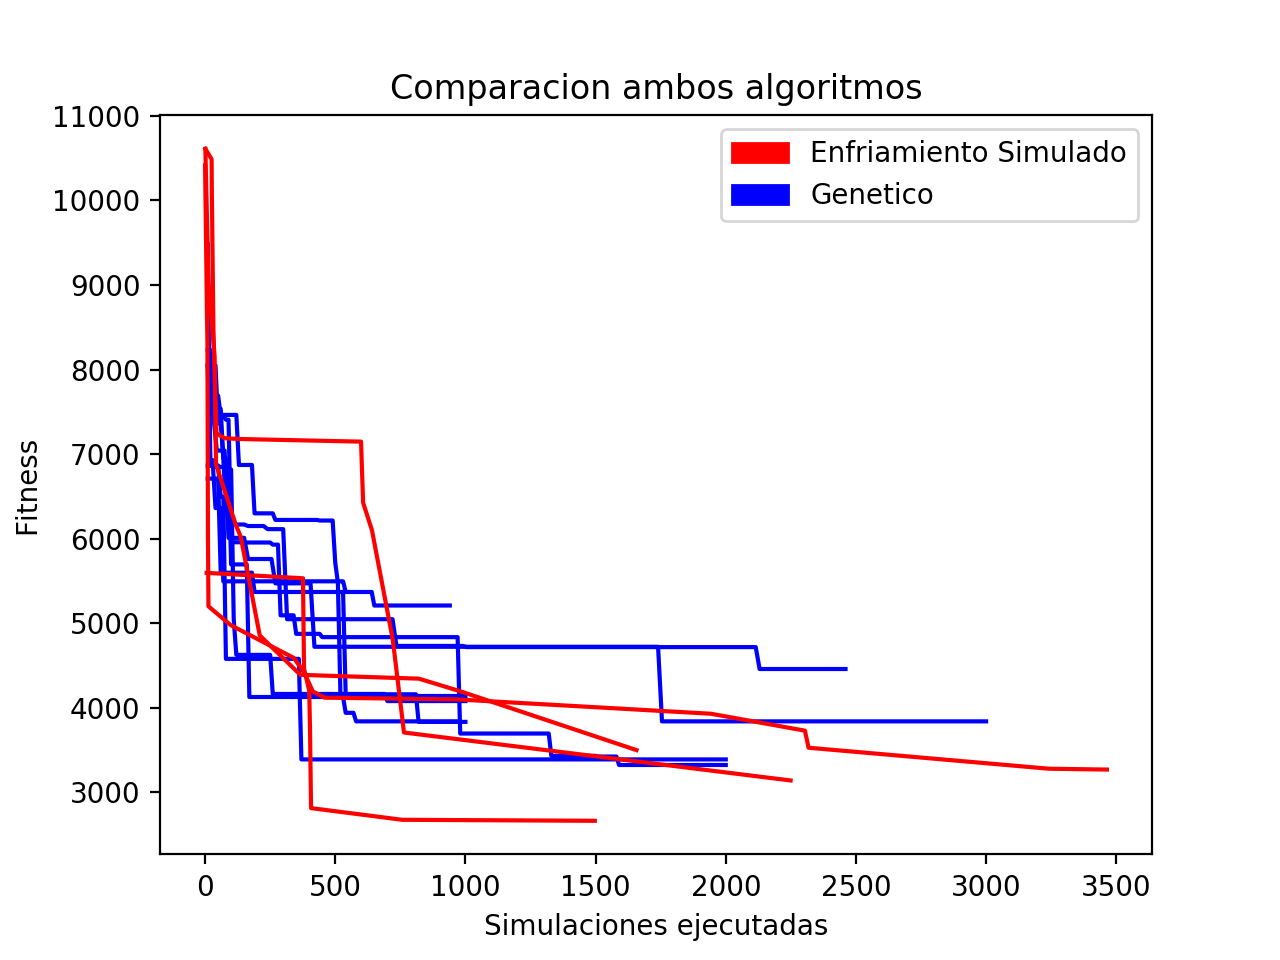
\includegraphics[scale=1]{images/comparacion_ambos}
	 			\label{fig:comparacion_ambos}
	 		\end{minipage}\hfill
	 	\end{figure}

	En este caso sí que se observan diferencias entre los dos algoritmos. El algoritmo genético tiene una media de resultados bastante peor que el enfriamiento simulado, utilizando una cantidad similar de recursos. 
	
\section{Conclusiones y trabajo futuro}
	Observando los resultados obtenidos podemos concluir que para este problema el algoritmo de enfriamiento simulado domina, y que ha obtenido un resultado mejor en casi todas las ejecuciones, y la media de fitness es mucho mejor que en el algoritmo genético. \\
	
	Además, para este problema es notable el hecho de hay muchos mínimos locales diferentes, y los algoritmos se suelen atascar en ellos y no mejorar (sobre todo en el genético). Por esta razón el resultado depende en gran medida de la configuración con la que se inicia el algoritmo (seed). \\

	Se me ocurren algunas posibles soluciones a estos estancamientos:
	
	\begin{itemize}
		\item 1. Utilizar enfriamiento simulado en los resultados del algoritmo genético
		\item 2. Utilizar enfriamiento simulado para generar el seed del algoritmo genético
		\item 3. Crear una variación del algoritmo genético, en el que varias 'familias' de individuos se van creando en paralelo, y cada x iteraciones se combinan (para obtener mayor variedad en los individuos)
	\end{itemize}
	
	Finalmente, cabe decir que este trabajo ha estado limitado por la velocidad de computación del fitness, en las simulaciones en el navegador. Si tuviera que volver a empezar, lo realizaría con una plataforma más adecuada para computaciones rápidas que me permitan realizar más experimentos. \\
	
	\section{Anexo: Interfaz desarrollada}
	La interfaz desarrollada se puede encontrar en la siguiente página web: \\ \href{http://personales.alumno.upv.es/fraruca/webgl/trabajo/?level=20}{http://personales.alumno.upv.es/fraruca/webgl/trabajo/?level=20} \\
	
	El funcionamiento es sencillo. En el centro de la pantalla aparecerá el nivel actual, al cual se puede jugar simplemente haciendo click en la posición y rotación donde se desea colocar la bola. Para empezar la simulación, hay pulsar la opción 'Run' dentro del menú 'Simulation' (arriba a la derecha). \\
	
	En el menú 'Optimizer' podemos encontrar las opciones para ejecutar un algoritmo de optimización (genetico o de enfriamiento simulado). Primero hay que elegir las opciones que se quieran utilizar, y luego darle al botón 'Start evolution' para comenzar. Una vez hecho esto, irán apareciendo poco a poco resultados en el menú 'Generations'. Se puede pulsar en uno de estos resultados para cargar la simulación deseada, que también se puede visualizar (otra vez en el menú 'Simulation'). \\
	
	Por último, en el menú 'Download' podemos descargar los resultados obtenidos de la optimización en nuestro ordenador, o cargar un archivo entrenado anteriormente. También podemos cargar archivos subidos al servidor de una lista, que pueden servir como ejemplo del funcionamiento del algoritmo ('Load from server').  
\begin{thebibliography}{50}
	\bibitem{arkanoid} 
	\href{https://es.wikipedia.org/wiki/Arkanoid}{https://es.wikipedia.org/wiki/Arkanoid}
\end{thebibliography}

\end{document}